\documentclass[a4paper,12pt,one side,titlepage]{report}


%en francais
\usepackage[T1]{fontenc}
\usepackage{lmodern}
\usepackage[utf8]{inputenc}
\usepackage[francais]{babel}



\usepackage{listings}
\usepackage{geometry}
\usepackage{graphicx}
\usepackage{eurosym}
\usepackage{url}
\usepackage{pdfpages}
\usepackage[acronym]{glossaries}
\usepackage{hyperref}
\usepackage{graphicx}
%\usepackage[top=2.5cm,bottom=2.5cm,left=2.5cm,right=2.5cm]{geometry}
%\hypersetup{pdfborder=0}




\newglossaryentry{firewall}
{
	name={firewall},
	description={Protection pour serveur}
}

\newglossaryentry{naxsi}
{
	name={naxsi},
	description={Un type de firewall}
}



\makeglossaries
\begin{document}
%\includepdf[pages = {1-1}]{./pdf/1stpage.pdf}
%\includepdf[pages = {1-1}]{./pdf/pagegarde.pdf}


\begin{titlepage}
\begin{center}

\textsc{\LARGE Licence ASRALL}\\[1.5cm]

\textsc{\Large Exposé technique}\\[5.9cm]

% Title
{ \huge \bfseries Fully Automatic Installation\\[1.9cm] }

% Author and supervisor
\noindent
\begin{minipage}{0.4\textwidth}
\begin{flushleft} \large
François \textsc{Dupont}
\end{flushleft}
\end{minipage}%
\begin{minipage}{0.4\textwidth}
\begin{flushright} \large
Florent \textsc{Fillion}
\end{flushright}
\end{minipage}

\vfill

% Bottom of the page
{\large \today}

\end{center}
\end{titlepage}


%Page table des matières
\tableofcontents

%Introduction
\chapter{Introduction}
\section{Objectifs}
\subsection{Définition}
\textit{Fully Automatic Installation} ou \textsc{FAI} est un logiciel libre, inspiré de son équivalent \textsc{Solaris}, \textsc{Jumpstart}. Il permet d'installer et de configurer un système d'exploitation Linux sur une ou plusieurs machines, en utilisant un infrastructure client serveur, de façon rapide et automatisé.

Il est à noter que \textsc{FAI} n'est pas interactif contrairement à d'autres logiciels remplissant sensiblement la même fonction. Ce logiciel est également considéré comme mature puisqu'il en est à sa 4\textsuperscript{ème} itération majeure (4.0) et est développé de façon continue depuis 1999.

\subsection{Utilité}
\textsc{FAI} s'adresse particulièrement aux administrateurs ayant à gérer un grand parc de machine sous Linux, que ce parc soit \textit{virtualisé} ou physique (et même des \textit{chroot}s).
On peut citer EDF qui a récemment utilisé FAI pour déployer son cluster/Super Ordinateur utilisant Debian. (classé dans les 50 premiers mondiaux au moment de moment de la son déploiement).
De nombreuses université comme le MIT l'utilisent pour gérer leur parc de machines GNU/Linux en comportant en général des centaines voire des milliers de postes clients.

\section{Histoire}
\textsc{FAI} est née en 1999 alors que Thomas \textsc{Lange}, Administrateur système experimenté sur Solaris a dû déployer plusieurs machines Debian/Gnu/Linux. Comme tous les administrateurs \textit{(compétents?)}, il déteste réaliser des choses répétitives et décide donc de s'atteler à l'automatisation du déploiement de machines Debian. Son projet est un succès, et est maintenant utilisé par de nombreuses administrations, écoles et entreprises.
Il est également, depuis, devenu développeur Debian.

Il a depuis été rejoint par d'autres développeurs, notamment Michael \textsc{Prokop} également développeur Debian et aussi mainteneur du dérivé minimaliste et orienté pour l'administration système \textsc{Grml}.
Et par Kerim \textsc{Gueney} collègue de \textsc{Lange} à l'Université de Cologne.

\subsection{La documentation}
On peut remarquer que ce projet est assez germano centré, tous les développeurs sont allemands ou bien travaillent dans une université allemande.
Cela ne pose pas de grands problèmes dans la mesure ou presque toute la documentation disponible est disponible en anglais.
Le problème est que cette dernière n'est pas maintenu très à jour (elle est souvent à jour de façon éclaté, wiki à jour mais le guide non, parfois l'inverse). Il existe cependant peu de \textit{talks}, ou documentation externe qui soit à jour ou pas en allemand.



\section{Concepts}
Cette partie pourrait avoir sa place dans le chapitre traitant de la technique à proprement parler, cependant, il nous semble essentiel d'exposer les principes fondamentaux (et simples une fois assimilés) de \textsc{FAI}. Il s'agit ici d'un survol, plus d'informations seront disponibles dans la partie réservé à la technique.


\subsection{Réseau}

\subsubsection{Classique}
Pour utiliser \textsc{FAI} vous devez avoir un réseau fonctionnel, avec un dhcp configuré, et un DNS fonctionnel. Moins classique, vous \textsc{devez} utiliser vos machines avec un démarrage réseau par PXE pour l'installation.

\subsubsection{Architecture Client Serveur}
\textsc{FAI} ne fonctionne qu'en mode client serveur (et pas par exemple en pair à pair). Avec 1 serveur pour N clients. Il faut cependant bien comprendre qu'un serveur peut délivrer plusieurs configurations (une Debian stable, une Debian testing, un Ubuntu ou même un RedHat), tout dépend de la configuration.

\subsection{Système}

\subsubsection{L'installation}
Une fois votre réseau en place et \textsc{FAI} installé sur un serveur vous pourrez éveiller le client (physiquement, wakeonlan) par PXE, le client ira ensuite s'identifier auprès du serveur. Notre client monte ensuite un partage NFS présent sur le serveur comme sa racine, une fois le noyau chargé, les scripts  d'installation FAI suivent leur cours et installe les configurations demandées par l'administrateur. Ces scripts peuvent inclure un partitionnement des disques ou bien formatage, l'installation de logiciels spécifique, gestion du RAID matériel, etc...

Il est possible d'utiliser un système de classe (programmation) pour créer des groupes d'ordinateurs similaires et ainsi facilité l'industrialisation de notre installation (il serait contre productif d'avoir à un profil par client). Il est possible d'utiliser plusieurs langages pour réaliser les scripts, bash, perl, ruby.

\subsubsection{La configuration}
La configuration doit être effectué avant de lancer une installation, pour rappel cette dernière n'est pas interactive, en revanche de nombreuses choses sont paramétrables en modifiant les bons fichiers et parfois quelques scripts.


\chapter{Technique}
Dans cette partie nous allons expliquer le fonctionnement plus précis de FAI en détaillant chaque composant majeur et dans la mesure du possible les différentes technologies disponibles pour réaliser ces actions ainsi que leurs principes.

\section{La base}


\subsection{DNS, DHCP et PXE}
Pour pouvoir utiliser \textsc{FAI} il faut avoir un DHCP et un DNS fonctionnel, bref rappel de leur utilité, le DHCP attribue une adresse IP à une adresse MAC, le DNS donne un nom à une IP.\\
La distribution \textsc{fai-server} propose d'utiliser le serveur iscdhcp une implémentation de référence maintenu par l'Internet Systems Consortium qui maintien également BIND \textit{(bref un truc sérieux)}. 
Pour une petite installation il est possible des la jouer \textit{old school} et d'utiliser le fichier /etc/hosts plutôt que d'utiliser un DNS sérieux, la documentation (et la logique aussi) nous dit que cela fonctionne pareil.

La configuration du DHCP est aisé même quand c'est la première fois et même avec un PXE coté client puisque la documentation interne fournie 


\subsection{Installer fai-quickstart}
De façon assez surprenant fai-quickstart (qui est indispensable à l'utilisation de FAI) n'est pas disponible sur la distribution FAI de base.\\
Ce paquet contient le serveur DHCP cité ci-dessus. Ainsi que le serveur tftp qui sera utilisé pour transférer notre distribution plus tard.

\subsubsection{TFTP}
\textsc{Trivial File Transfert Protocole} est un protocole de transfert de fichier qui utilise  le protocole UDP (rappelons qu'UDP est un protocole de la couche 4 du modèle OSI, la couche transport. Contrairement à TCP, UDP ne fait pas de négociations et ne vérifie pas non plus l'intégrité des données qu'il délivre). \\
Ce protocole est généralement utilisé pour le streaming vidéo/audio ou encore les jeux en réseaux, plus généralement pour toutes les applications où l'exactitude du message est négligeable devant la nécessité de réactivité. Avec \textsc{FAI} on tire partie du la capacité d'UDP à envoyer très vite beaucoup de données de petites taille. Ce gain de vitesse par rapport à tcp est lié à l'absence de handshake.
L'expérience montre que l'UDP utilisé sur un réseau local de \textsc{qualité} ne présente presque jamais de problèmes d'intégrité.\\
TFTP en lui même est une version simplifié de FTP (pas de gestion de droits pas de possibilité de ls ou delete dans un répertoire) il est conçu pour la mise à jour ou la copie simple de fichiers.



\subsection{NFSROOT}


\subsection{configuration de bases}


\section{Configurations avancées et options en tout genres}
On peut configurer de nombreuses choses avec \textsc{FAI}

\subsection{Le Debian mirror}
Une des astuces facile voire évidente est l'installation d'un miroir Debian en local (que ce soit ou non sur notre fai-server)




\chapter{Alternatives}

\section{Jumpstart}
Jumpstart a été créé par Sun Microsystems, qui fut ensuite racheté en 2009 par Oracle Corporation. C'est un outil permettant d'automatiser l'installation d'une ou plusieurs machines utilisant Solaris comme système d'exploitation.\\
La configuration de Jumpstart s'effectue à l'aide de plusieurs fichiers :\\
\begin{itemize}
  \item Le fichier \textit{profile} qui définit les partitions de disques.
  \item Les fichiers \textit{rules} et \textit{rules.ok} qui définissent les règles correspondant à un profil particulier de client à installer.
  \item Des scripts s'exécutant avant et après l'installation de la machine cliente.
  \item Le fichier \textit{sysidcfg} qui définit les informations de configuration du client, comme par exemple son nom d'hôte, son adresse IP, etc...
  \item Le fichier \textit{/etc/bootparams} qui est utilisées par les machines clientes pour démarrer.
  \item Le fichier \textit{/etc/ethers} qui contient les mappages d'adresses MAC pour les clients.\\
\end{itemize}

Lors de l'installation, le programme Jumpstart va tenter de faire correspondre le sytème à installer aux règles définies dans le fichier \textit{rules.ok}. Il lit donc ces règles, de la première à la dernière. Lorsque qu'une correspondance est établie entre un système et une règle, le programme JumpStart interrompt la lecture du fichier \textit{rules.ok} et commence l'installation du système d'après le profil correspondant à la règle associée.\\
\begin{center}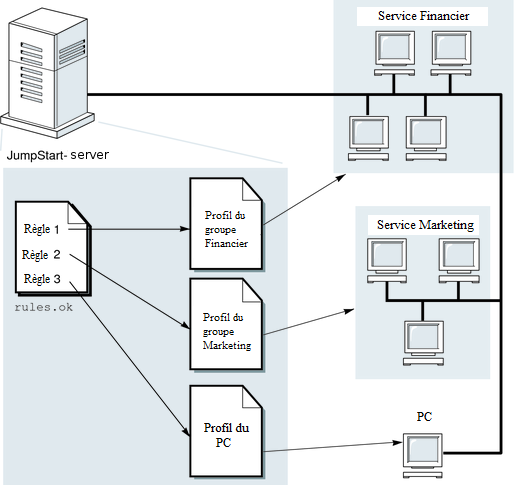
\includegraphics[scale=0.7]{./img/jumpstart2.png}\end{center}
\vspace{1em}
Un serveur DHCP peut également être mis en place sur le serveur Jumpstart afin d'attribuer automatiquement une configuration IP aux machines clientes.\\\\
Voici un schéma représentant brièvement les requêtes effectuées entre les clients et le serveur lors du démarrage de l'installation :\\
\begin{center}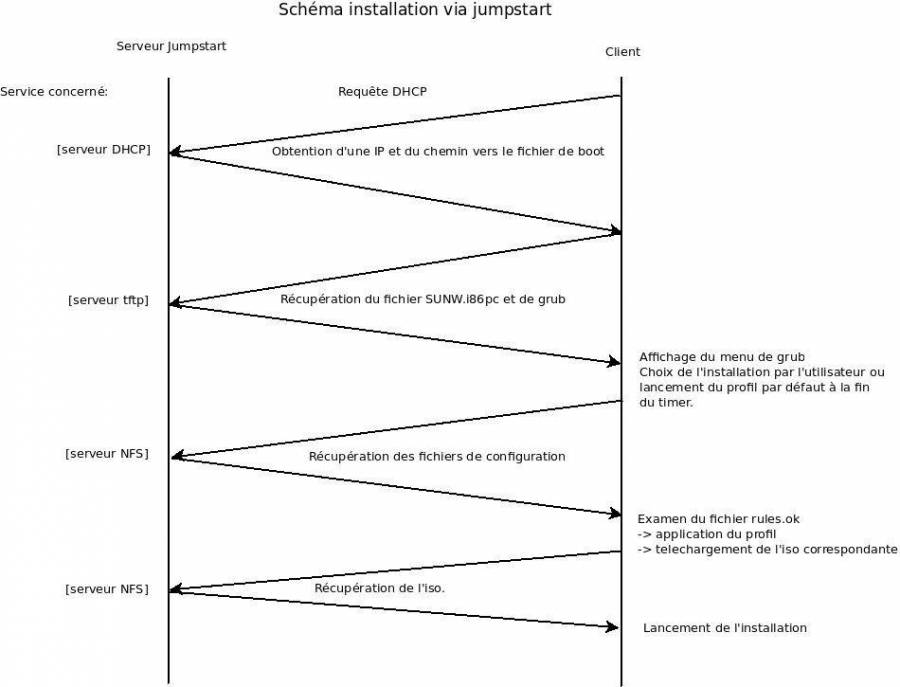
\includegraphics[scale=0.4]{./img/jumpstart.jpeg}\end{center}
\subsubsection{Configuration du serveur Jumpstart}
Voici la liste des tâches à effectuer lors de la préparation à une installation JumpStart :\\
\begin{itemize}
  \item Créer un répertoire JumpStart\\
  \item Ajouter des règles pour chaque groupe dans le fichier \textit{rules} :\\
Chaque règle définit un groupe d'après un ou plusieurs attributs système. La règle lie chaque groupe à un profil.\\
  \item Créer un profil pour chaque règle :\\
Un profil est un fichier texte qui définit l'installation du logiciel Solaris, et indique par exemple le groupe de logiciels devant être installé sur un système. À chaque règle correspond un profil qui définit la procédure d'installation du logiciel Solaris sur un système. Ce profil est utilisé dès qu'une correspondance est établie entre une règle et un système déterminés.\\Généralement, on définit un profil pour chaque règle. Le même profil peut toutefois être utilisé dans plusieurs règles.\\
  \item Valider le fichier \textit{rules} :\\
Le fichier \textit{rules.ok} est une version générée du fichier \textit{rules} qu'utilise JumpStart pour détecter le système à installer avec un profil. Le fichier \textit{rules} se valide par l'intermédiaire d'un script \textit{check}.
\end{itemize}

\section{Kickstart}
Kickstart a été créé par RedHat afin d'automatiser l'installation de Fedora et Red Hate Enterprise Linux. Sa configuration s'effectue dans un fichier kickstart \textit{ks.cfg} unique contenant une liste d'éléments, chacun identifié par un mot-clé.\\Ces éléments correspondent aux réponses à toutes les questions qui devraient normalement être posées lors d'une installation typique.\\
Ce fichier peut être créé manuellement en partant d'un fichier vierge puis en écrivant les directives une par une.\\

Cependant, et contrairement à FAI, il existe une interface utilisateur graphique, "Kickstart Configuration", permettant ainsi une configuration plus simple puisque il n'est pas nécessaire de se rappeler de la syntaxe exacte du fichier kickstart à configurer.\\\\
Il suffit donc de suivre les étapes les unes après les autres afin de configurer petit à petit le fichier en question :\\
\begin{center}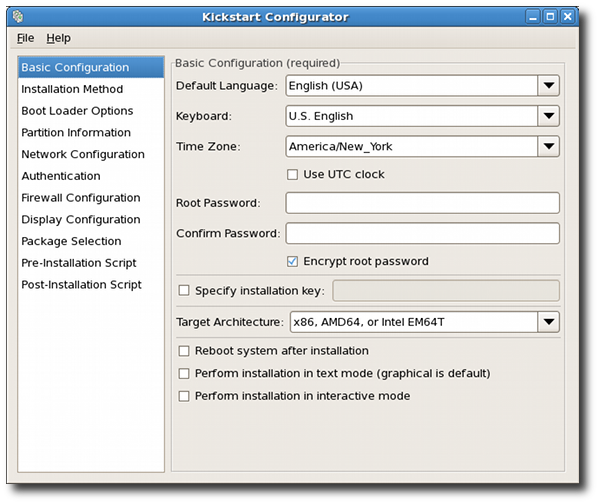
\includegraphics[scale=0.5]{./img/kickstart.png}\end{center}
\vspace{1em}
Si l'on souhaite effectuer une installation plus fine et personnalisée, il est également possible de rajouter des scripts d'installations via l'interface graphique.
Ces scripts peuvent être exécuté avant (Pre-Installation Script) ou après l'installation (Post-Installation Script) :
\begin{center}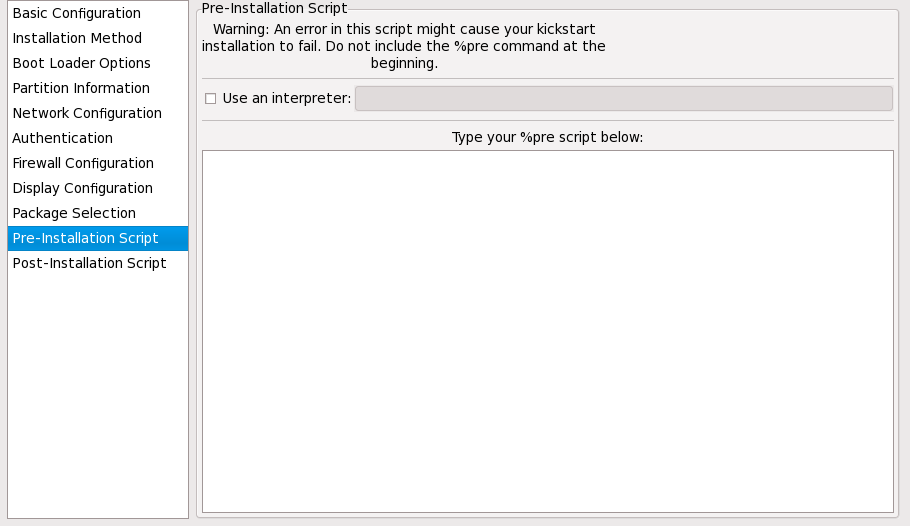
\includegraphics[scale=0.5]{./img/kickstart2.png}\end{center}
\vspace{1em}
Si l'on souhaite par exemple effectuer manuellement une configuration réseau dans le fichier kickstart, il suffira d'inclure le script dans la zone de texte prévue à cet effet.\\
En effet, avant le début de l'installation, le fichier kickstart est analysé afin des détecter les différentes commandes à exécuter. Si une configuration réseau est détectée dans le fichier kickstart, avant que la section "Network Configuration" soit traitée, la configuration réseau sera prioritaire et prise en compte.\\
Pour spécifier un langage de script particulier à utiliser pour exécuter le script, il suffit de sélectionner l'option "use an interpreter" et d'entrer le langage souhaité, par exemple \textit{/usr/bin/python2.7}.\\

Une fois la configuration terminée, il est tout de même possible de consulter le fichier kickstart avant de le sauvegarder.

Il suffit ensuite de placer le fichier \textit{ks.cfg} généré sur le support de démarrage souhaité, puis de booter la machine cliente sur ce même support de démarrage. Une commande de démarrage spéciale est à taper à l'invite de démarrage. Le programme d'installation va ainsi rechercher si un fichier kickstart est présent, puis va s'en servir pour procéder à l'installation du système.

\section{Rembo}
Rembo est le successeur de BPBatch. Il a été créé par "Rembo Technology", une société suisse spécialisée dans les outils de gestion applicative et de virtualisation de serveurs, qui fut ensuite rachetée en 2006 par IBM. Rembo est un environnement de déploiement d'applications qui permet d'installer rapidement et en même temps, n machines du même type. Il peut s’exécuter sur Windows, Linux ou encore FreeBSD et s’appuie sur un serveur DHCP. Les machines clientes doivent donc supporter PXE et auront dont exactement la même installation.\\

L'installation s'appuie sur l'utilisation d'une platine virtuelle, sur laquelle on sélectionne les programmes à installer. La procédure est ensuite entièrement automatique, et personnalisable à l'infini. Une machine virtuelle est créée à chaque installation puis est effacée lorsque le processus est terminé.\\
..............................................

\section{Clonezilla}
Clonezilla est une logiciel libre créé par le laboratoire de recherche NCHC pouvant être utilisé sur plusieurs systèmes d'exploitations différents tel que Linux, Windows ou encore MAC OS X par exemple. Il permet de créer une image de sauvegarde d'un disque dur ou d'une ou plusieurs partitions, pour ensuite la restaurer ou la cloner sur une (unicast) ou plusieurs machines clientes (multicast).\\
Il existe deux version de Clonezilla, "Clonezilla Live" et "Clonezilla Server" :\\
\begin{itemize}
  \item Clonezilla Live est utilisé par l'intermédiaire d'un Live CD, (ou clé usb également). Il permet à l'utilisateur d'effectuer directement depuis la machine une sauvegarde d'un disque ou d'une partition, une restauration d'une image depuis un disque, ou encore un clonage d'une image vers un autre disque. Cepedendant, ces actions ne peuvent s'effectuer que sur une seule machine à la fois puisque le Live CD est obligatoire.\\
  \item Clonezilla Server (ou Clonezilla SE) est utilisé depuis un serveur et autorise plusieurs postes à se connecter simultanément par l'intermédiaire d'un réseau commun. Il n'y a donc pas besoin de Live CD ce qui permet d'effectuer des sauvegardes/restaurations/clonages sur plusieurs machines à la fois. Un serveur DRBL (Diskless Remote Boot in Linux) est utilisé ce qui permet aux stations esclaves concernées d'effectuer un démarrage PXE.
\end{itemize}
\begin{center}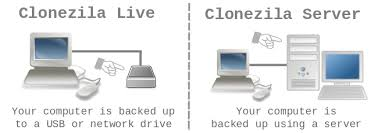
\includegraphics[scale=0.9]{./img/clonezilla.jpeg}\end{center}
\vspace{1em}
\subsubsection{Le serveur DRBL}
DRBL permet de mettre à disposition un environnement système léger pour les machines clientes et intègre Clonezilla.\\
Il est donc utilisé, le plus souvent, pour le clonage massif de postes de travail et le déploiement rapide de salles informatiques. Il s'appuie exclusivement sur des logiciels libres tel que \textit{partimage}, \textit{ntfsclone} ou encore \textit{partclone} pour cloner des disques/partitions, et utilise également \textit{udpcast} pour transférer des données simultanément sur plusieurs destinations via le réseau (unicast/broadcast/multicast).

DRBL supporte les systèmes de fichiers ext2, ext3, ext4, reiser4, xfs, jfs, fat, ntfs, hfs+, ufs, vmfs3 ainsi que LVM2. Les bootloader syslinux et grub peuvent être installés.

\subsubsection{Principe général de fonctionnement de Clonezilla Server}
\vspace{1em}
\begin{center}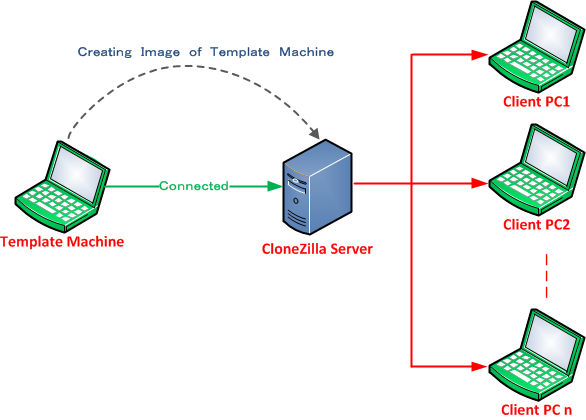
\includegraphics[scale=0.7]{./img/clonezilla2.png}\end{center}
\vspace{1em}
Le serveur Clonezilla a besoin d'une image type, afin qu'il puisse s'en servir par la suite comme référence pour sauvegarder, restaurer ou cloner cette même image sur les différentes machines clientes.\\
Lors d'un clonage par exemple, une fois l'image disponible sur le serveur, celui-ci va la copier simultanément sur les différentes machines clientes, via le réseaux (PXE).

\chapter{Conclusion}

\chapter{Sources}
\begin{itemize}
  \item http://fai-project.org/\\
  \item http://www.markus-gattol.name/ws/fai.html\\
  \item https://github.com/faiproject/fai\\
  \item https://www.linux-magazine.com/w3/issue/100/066-071\_FAI.pdf\\
  \item http://grml.org/\\
  \item https://docs.oracle.com/\\
  \item https://access.redhat.com/documentation/\\
  \item http://http://clonezilla.org/\\
  \item https://www.projet-plume.org/fiche/drblclonezilla\\
\end{itemize}


\end{document}
